\section{Umsetzung}
\subsection{Technologie und Plattform}
In der Problembeschreibung zu dieser Arbeit wurden die Anforderungen an eine SmartHome Lösung diskutiert. In der anschliessenden Marktanalyse wurde openHAB als Grundlage zur Umsetzung unseres Projekts evaluiert. OpenHAB erfüllt die geforderten Kritierien, wie Herstellerunabhängigkeit, Installierbarkeit und Flexibilität. 
Für unser Projekt werden verschiedene Technologien bzw. Platformen eingesetzt. Auf der Clientseite, im SmartHome, wird openHAB mit verschiedenen Bindings eingesetzt. Cloudseitig wird MS Azure Cloud zur Persistierung von Events verwendet.

\subsection{openHAB}
Das System openHAB wird eingesetzt, um verschiedene Home-Automatisierungssysteme unter einen Hut zu bringen. Um dies zu realisieren bietet openHAB eine grosse Anzahl von Bindings mit, mit denen die verschiedenen Systeme angesprochen werden können.

\subsubsection{Module}
OpenHAB ist durch OSGi-Bundles modular aufgebaut und binhaltet folgende Komponenten:

\begin{figure}[H]
	\centering
		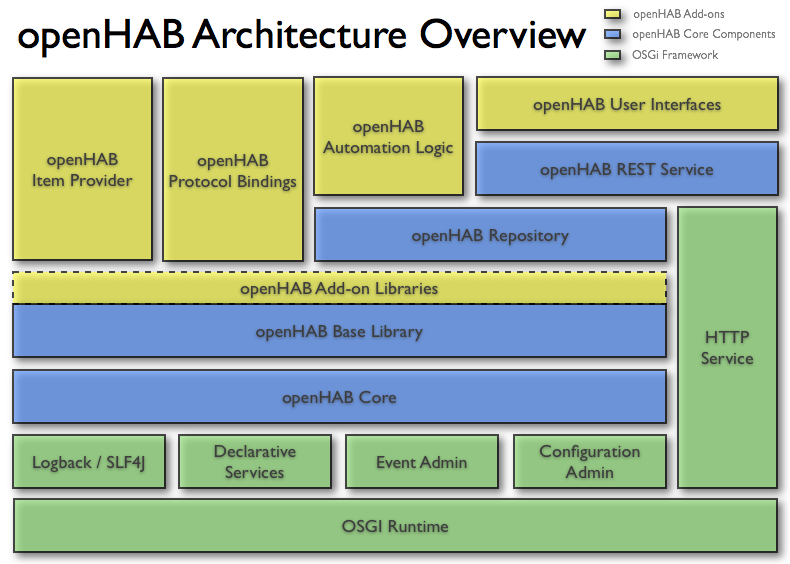
\includegraphics[scale=0.45]{report/img/openHAB_architecture}
	\caption{openHAB Architektur}
	\label{fig:ohArch}
\end{figure}


\subsubsection{Kommunikation}
Der Basisservice von openHAB stellt der Event Bus dar. Über diesen Bus werden Events zwischen den verschiedenen Bundles gesendet. Die Events sind entweder Commands, welche eine Aktion ausführen, oder Status-Updates, welche Statusänderungen der Devices beinhaltet. \\
Durch den Einsatz dieses EventBus wird die Kopplung reduziert und können somit einfach ausgetauscht werden. \\
Für die Verwaltung der verschiedenen Status ist das Item Repository zuständig, welches permanent den Event Bus auf Status-Updates abhört und die Änderungen ins Repository schreibt. Falls auf einem GUI ein Status eines Devices angezeigt werden soll, kann dazu das Item Repository abgefragt werden.\\
Das Repository persistiert die Status und ist somit auch nach einem Neustart verfügbar.

\begin{figure}[H]
	\centering
		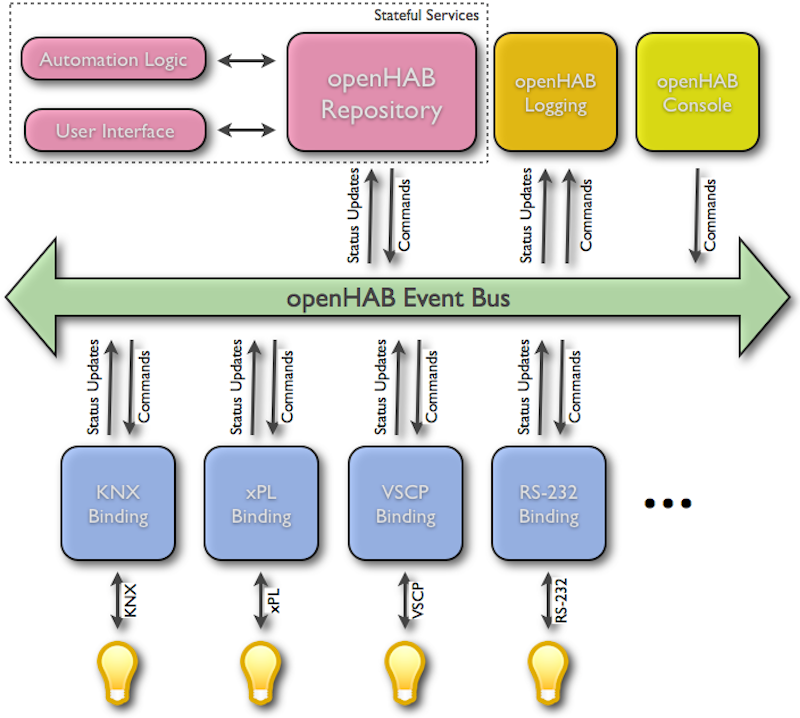
\includegraphics[scale=0.4]{report/img/communicationOH}
	\caption{Kommunikation openHAB}
	\label{fig:ohComm}
\end{figure}

\subsubsection{Bindings}
Ein Binding ist eine Verbindung zwischen dem Event Bus und den externen Systemen. Diese Verbindungen sind aufgrund der verschiedenen Technologien verschieden. Dadurch muss für jede Technologie ein eigenes Binding geschrieben werden. Für einige Systeme sind Bindings vorhanden, die einzeln heruntergeladen und als «Add-on» installiert werden können.
Die Bindings stellen nur sicher, dass Events zwischen Event Bus und den jeweiligen Devices ausgetauscht werden können. Sie müssen sich also nicht um Statusänderungen oder ähnliches kümmern, da dies durch das Item Repository übernommen wird. \\
Alle momentan verfügbare Bindings sind unter folgendem Link zu finden: \url{https://github.com/openhab/openhab/wiki/Bindings}

\pagebreak

\subsection{Installation openHAB}



\subsection{Deploymentübersicht}

\subsubsection{Binding Azure}
\begin{figure}[h!]
	\centering
		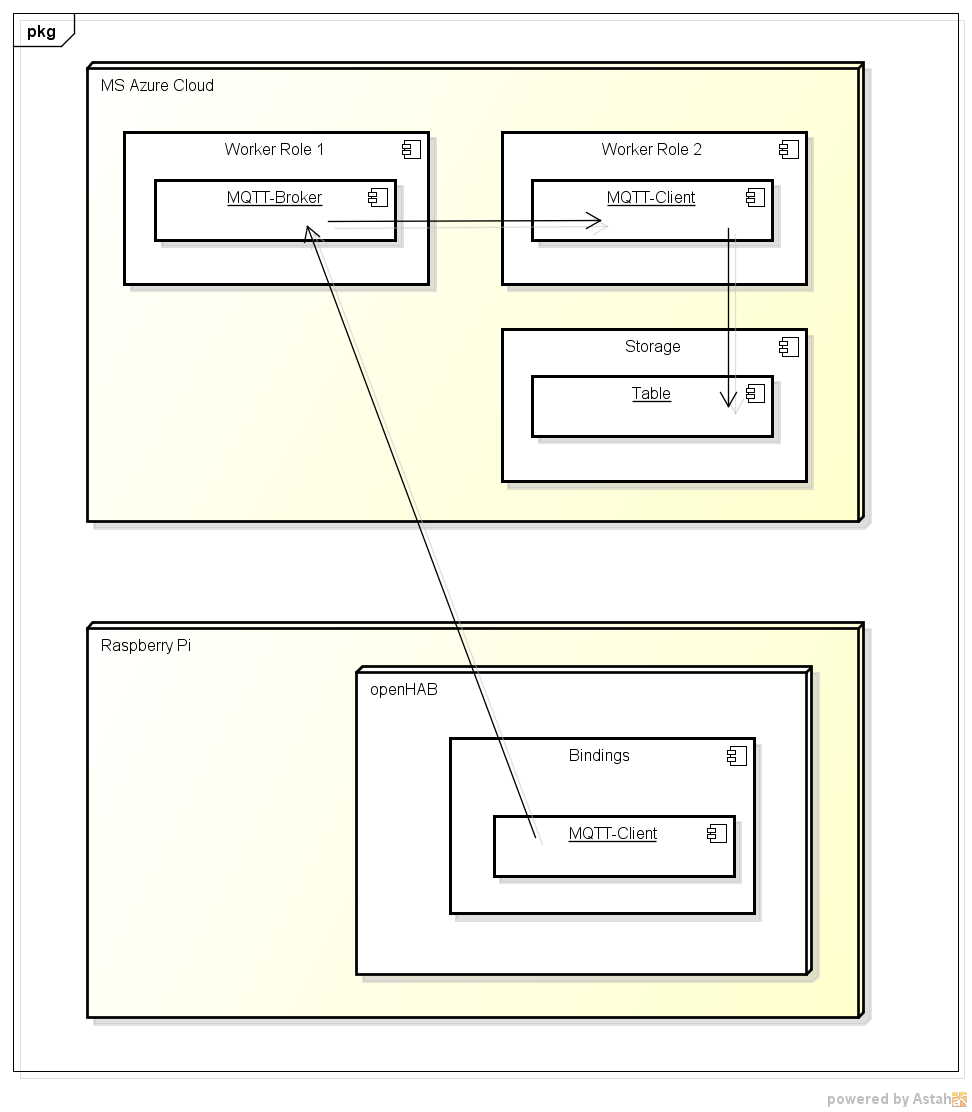
\includegraphics[scale=0.5]{report/img/deployment_binding_azure}
	\caption{Binding Azure Cloud}
	\label{fig:deploymentAzure}
\end{figure}

\subsection{MQTT}
MQTT steht für «Message Queue Telemetry Transport» und ist ein Nachrichten-Protokoll, das speziell für IOT-Anwendungen konzipiert wurde. Es setzt auf dem TCP/IP Stack auf und wird für den Nachrichtenaustausch zwischen verschiedenen, verteilten Maschinen verwendet. \\
Das Protokoll wurde speziell für Systeme designt, die über wenig Speicherplatz und kleiner Netzwerk-Bandbreite verfügen, was bei IOT-Anwendungen meist der Fall ist.

\subsubsection{Funktionsweise}
MQTT folgt dem Prinzip «Publish/Subscribe», sprich Clients können bestimmte Topics abonnieren. Wenn Messages auf dieses Topic gesendet werden, leitet der Broker diese an alle interessierten Clients weiter. \\
In Bezug auf erstellen von Topics agiert der Broker passiv. Das bedeutet, Clients können sich auf beliebigen, selber defnierte, Topics registrieren. Wenn aber niemand auf dieses Topic publiziert, wird der Client nie eine Message erhalten.

\begin{figure}[h!]
	\centering
		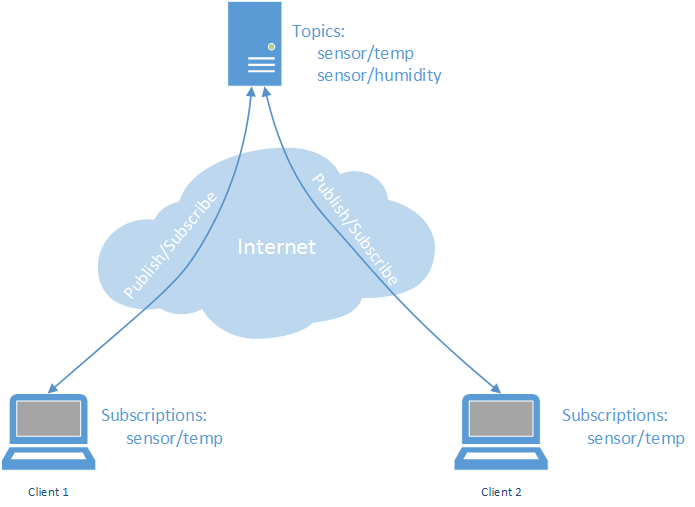
\includegraphics[scale=0.6]{report/img/mqttFunktionsweise}
	\caption{Funktionsweise MQTT}
	\label{fig:deploymentAzure}
\end{figure}

\subsubsection{Broker}

\textbf{Zertifizierungsstelle/Server-Zertifikat} \\
Da die MQTT-Verbindung verschlüsselt werden soll, müssen verschiedene Zertifikate erstellt werden. Das erstellte Server-Zertifikat muss von einer CA (Certification Authority) signiert werden. Da ein gültiges Zertifikat nicht entgeltlich erworben werden möchte, wird eine eigene Zertifizierungsstelle erstellt. OpenSSl bringt da alle nötigen Mittel für die Erzeugung eines CAs mit. Dies bringt den Nachteil mit, dass Computersysteme diesem Zertifikat nicht automatisch trauen, daher muss dann das Zertifkat von Hand dem Certificate Storea als «Trusted Root Certification Authority» hinzugefügt werden. \\

Nachdem die Zertifizierungsstelle erfolgreich generiert wurde, kann das Server Zertifikat erstellt werden. Anschliessend muss dieses Server Zertifikat von der eben erstellten Zertifizierungsstelle signiert werden.

Da sowohl die Zertifizierungsstelle, als auch das Server-Zertifikat auf dem gleichen Computer erstellt werden, muss darauf geachtet werden, dass bei der Erzeugung unterschiedliche Parameter gesetzt werden. Die betroffenen Parameter sind zum Beispiel «Locality Name», «Organizational Name», «Organizational Unit» etc. Falls hier dieselben Werte eingetragen werden, schlägt die Signierung des Serverzertifikates fehl. \\
Weiter muss beachtet werden, dass im Server-Zertifikat der «Common Name» dem FQDN (Fully Qualified Domain Name) des Servers entspricht, auf dem der MQTT-Broker laufen soll. Wird hier beispielsweise nur der Hostname eingetragen, schlägt die Überprüfung des Zertifikates fehl, da sich der CN vom FQDN des Servers unterscheidet.

\textbf{Installation und Konfiguration des Brokers} \\
Wie bereits im Lösugnskonzept erarbeitet, wird als MQTT-Broker «Mosquitto» eingesetzt. Der Broker kann als Binary installiert und über die Commandline gestartet werden.
Nach der Standard-Installation muss der Broker Konfiguriert werden. Dazu wird das File «mosquitto.conf» bearbeitet.
\\Folgende Parameter müssen editiert werden:

\begin{tabularx}{\textwidth}{lX}
		\textbf{Parameter} & \textbf{Erklärung}
		\\ \hline
			bind\_address \tbd &
			IP-Adresse, an den der Default-Listener gebunden wird.
		\\ \hline
			port 8883 &
			Port, auf den der Default-Listener hören soll. Wenn er nicht speziell definiert wird, hört der Listener per Default auf den Port 1883. Da aber mit TLS verschlüsselt wird, muss dieser von Hand auf den dafür vorgesehenen Port 8883 gesetzt werden.
		\\ \hline
			cafile \tbd &
			Hier wird der Pfad eingetragen für das zuvor erstellte CA-Zertifikat.
		\\ \hline
			certfile \tbd &
			Hier wird der Pfad eingetragen für das PEM-Encodete Server Zertifikat.
		\\ \hline
			keyfile \tbd &
			Hier wird der Pfad eingetragen für das PEM-Encodete Keyfile.
		\\ \hline
			tls\_version tlsv1 &
			Diese Option definiert die zu verwendende TLS-Version. Für Openssl (Version 1.0.2) wird tlsv1 verwendet.
		\\ \hline
\end{tabularx}

\subsubsection{Client (Azure Worker Role)}
Wie die Abbildung \ref{fig:systemView} (Systemübersicht) zeigt, befindet sich nebst dem Broker auch ein Client, in form einer Worker Role, in der Cloud. Die Worker Role abonniert alle Topics und persistiert die Messages im Table bzw. Blob-Storage.

In der \lstinline!OnStart()!-Methode der Worke Role werden zu erst die Referenzen zum Table- und Blob-Storage erzeugt. \\
Danach wird die Verbindung zum MQTT-Broker hergestellt, die Topics definiert, die er abonnieren möchte und der QoS-Level gesetzt. \\
Damit der Client benachrichtigt wird, wenn eine Message eintrifft, wird der Eventhandler \lstinline!client_MqttMsgPublishReceived()! definiert. Die Methode muss die gleichen Parameter entgegennehmen, wie die Delegate-Methode. Das ist einerseits der Sender (Object) und die Event-Argumente. Damit der Eventhandler beim Eintreffen einer Message aufgerufen wird, muss dieser auf dem Event registriert werden: \\ \lstinline!client.MqttMsgPublishReceived += client_MqttMsgPublishReceived;! 

\begin{lstlisting}[style=csharp]
public override bool OnStart()
{
  setupStorageConnections();
  MqttClient client = new MqttClient(
            				"mqttbrokerba.cloudapp.net",
               				8883, true, null
               			  );
  client.MqttMsgPublishReceived += client_MqttMsgPublishReceived;
  client.Connect(Guid.NewGuid().ToString(),
  				 "mosquitto",
  				 "baIOT_mq++"
  				 );
  string[] topics = { "openhab/+" };
  byte[] qos = { MqttMsgBase.QOS_LEVEL_EXACTLY_ONCE };
  client.Subscribe(topics, qos);

  return result;
}
\end{lstlisting}

Im Eventhandler wird dann schlussendlich die Logik zur Persistierung eingefügt. 












